\def\DevnagVersion{2.15}\documentclass[11pt]{article}
\usepackage{acl2014}
\usepackage{times}
\usepackage{url}
\usepackage{latexsym}
\usepackage{devanagari}
\usepackage{graphicx,subfigure}
\usepackage{float}
\usepackage{pdfpages}


%\setlength\titlebox{5cm}


\title{Word Vector Averaging: Parserless Approach to Sentiment Analysis}

\author{Pranjal Singh \\
  Dept. of Computer Science \& Engg. \\
  IIT Kanpur \\
  {\tt spranjal@iitk.ac.in} \\\And
  Amitabha Mukerjee \\
  Dept. of Computer Science \& Engg. \\
  IIT Kanpur \\
  {\tt amit@cse.iitk.ac.in} \\}

\date{}

\begin{document}
\maketitle
\begin{abstract}
 In recent years, distributional compositional semantics or word vector models
have been proposed to capture both the syntactic and semantic similarity
between words.  Since these can be obtained in an unsupervised manner, they
are of interest for under-resourced languages such as Hindi.  We test the
efficacy of such an approach for Hindi, first by a subjective overview which
shows that a reasonable measure of word similarity seems to be captured in
the model.  We then apply it to the standard problem of sentiment analysis,
for which several small database exist in Hindi.  This requires some
mechanism for dealing modeling larger strings given the vectors for its
words, and several methods - additive, multiplicative, or tensor neural
models, have been proposed.  Here we find that the simplest - an additive
average, results in an accuracy of 91.1\% for an existing product review
dataset and and 89.9\% for a Hindi movie review dataset; both numbers are
nearly 10\% higher than earlier state of the art.  The results suggest that
at the very least, it would be important to explore further with such methods
for other applications.
\end{abstract}


\section{Introduction}
Over a period of nearly a millenium, there was an extensive debate between
Indian grammarians on whether sentence meaning accrues by combining word
meanings, or whether words gain their meanings based on the context they
appear in~\cite{Matilal:90}.  The former position, that
meaning is {\em compositional}, has been associated with the fregean
enterprise of semantics, whereas recent models, building on large corpora of
text (and associated multimedia) a large degree of success has accrued to
models that attempt to model word meaning based on their linguistic context
(e.g. ~\cite{Landauer:97}).  The latter line has resulted in strong improvements in several NLP tasks using word vectors~\cite{Collobert:08,Turian:10,Mikolov:13a,Socher:13}. 
The advantage of these approaches is that they can capture both the syntactic
and the semantic similarity between words in terms of their projections onto
a high-dimensional vector space; further, it seems that one can tune the
privileging of syntax over semantics by using local as opposed to large contexts~\cite{Huang:12}. 

For resource-poor languages, these approaches have the added lure
that many of these methods can work directly with large raw text corpora,
and avoid contentious issues such as decicing on a POS-tagset, or expensive
human annotated resources such as treebanks.  For Indian languages therefore,
it would be natural to seek to apply such methods.  At the same time, it must
be noted that many approaches combine POS-tags and even parse tree structures
into the models for higher accuracies in specific tasks. 

Vector models for individual words are obtained via distributional learning, the
mechanisms for which varies from document-term
matrix factorization~\cite{Landauer:97},
various forms of deep learning~\cite{Collobert:08,Turian:10,Socher:13}, 
optimizing models to explain co-occurrence constraints
~\cite{Mikolov:13a,Pennington:14},etc. Once the word vectors have been assigned, similarity between words can
be captured via cosine distances. 

One difficulty with this approach is that how words should be
combined into larger phrases is not clear.  In past work,
inverse-similarity weighted averaging appears
to work to some extent even for complex tasks such as essay grading \cite{Landauer:03},
but multiplicative models (based on a reducing the tensor products of the
vectors) appears to correlate better with human
judgements~\cite{Mitchell:08,Socher:13}.
Another complexity in composition is that composing words across phrasal
boundaries are less meaningful than composing them within a phrase - this has
led to models that evaluate the nodes of a parse tree, so that only coherent
phrases are
evaluated~\cite{Socher:13}. 

\subsection{Sentiment Analysis}

In order to evaluate the efficacy of the model, we apply it to the task of
sentiment analysis.
Here the problem is that of identifying the polarity of sentences such as 
\begin{itemize}
\item Positive: {\dn rA\8{m} n\? khAnF kF r\327wtAr khF{\qva} Tmn\? nhF{\qva} dF} [Ramu didn't allow the pace of the story to subside]
\item Negative: {\dn pd\?{\qvb} pr EdKAyA jA rhA KO\327w Esn\?mAGr m\? nhF{\qva} psr pAtA} [The horror shown on the screen didn't flip out in the theater]
\end{itemize}
See (Liu et al. 2012) for a recent survey.

This is a problem that has attracted reasonable attention in Hindi (see section~\ref{sec:related}), since most sentiment
analysis is oriented towards semantics, and one may bypass the syntactic
processing which for Hindi is still poor.   Methods that have been used
are largely based on assigning a sentiment effect for individual words, and
then combining these in some manner to come up with an overall sentiment for
the document.  Such methods, that ignore the order of the words have been
criticized since the import of a sentence can change completely simply by
re-arranging the words, which would leave the results unaffected.
It is to improve such situations that several groups have attempted to model
the composition of words into larger contexts~\cite{Mikolov:13c,Socher:13,Johnson:14}.
However, most of the work on sentiment analysis in Hindi has not attempted to
form richer compositional analyses.   For the two corpora used here, the 
best results, obtained by combining a sentiment lexicon with hand-crafted analysis (e.g. modeling negation and "but" phrases), reach an accuracy of about 80\%.  

In this work, we first learn a distributional word vector model
based on the wikipedia Hindi corpus, and then we use this to discern
the polarities in on two existing corpora of movie and product reviews.
To our own surprise, we find that even a simple additive composition model
improves the state of the art in this task significantly, to just
shy of 90\% (a gain of nearly 10\%).
At the same time, when applied to English
the system does respectably, but well behind the very best
models that attempt more complex composition marginally. 
So the question arises as to whether the very significant gains in
Hindi are due to some quirk in the 
dataset, or could it be that Hindi word vectors are particularly informative,
maybe because of the much more highly inflected nature of its
surface forms.  Also, if the results are not corpus-specific, it also raises
the possibility that word vector methods may result in significant gains in
other similar problems for Hindi. 
 
% For example, the sentences below give a brief idea of what positive and negative sentiment means.
% \begin{itemize}
% \item Positive: {\dn yh EPSm aQCF h\4}
% \item Negative: {\dn yh smAn b\7{h}t KrAb h\4}
% \end{itemize}
% \footnotetext{en.wikipedia.org/wiki/List\_of\_languages\_by\_number\_of\_native\_speakers}
% Majority of the existing work in this field is in English (Pang and Lee, 2008).
% Our model uses word vector averaging to build document vectors which constitute a feature set for our SVM classier. We have used skip-gram model (Mikolov et al., 2013b) for building word vectors because deep network model of Collobert et al.(2008) takes too much time for training. Also the word embeddings obtained by them are not as good as those obtained by Mikolov et al.(2013b). On NER task, skip-gram obtained F1-score of 93.1 while CW obtained F1-score of 92.2. We have also experimented with tf-idf for building our feature set. Our model shows slight improvement in performance if we filter out certain corpus based stop words. This is a first attempt to use word vectors for sentiment analysis in Hindi. Word vectors capture both semantic and syntactic information for a given corpus. Words which are semantically and syntactically related tend to be closer in high-dimensional space.\\
% This paper is organised as follows. Section 2 presents related work in the field of sentiment analysis. Section 3 describes our approach in detail. Experiment setup and datasets are described in Section 4. Section 5 looks into the results we have obtained and compares them with the results of existing models. Section 6 concludes and presents the future work.

\section{Related Work}
\label{sec:related}
Sentiment analysis is an important task in the field of NLP. SemEval-2014 had tasks from the domain of sentiment analysis which included aspect based sentiment analysis. It has emerged as one of the most important NLP tasks these days. Liu et al. (2012) and Pang et al. (2008) have provided a comprehensive literature of work done in this area. These days the focus has shifted mainly on microblogs(mainly Twitter) and reviews. Mohammad et al.(2013) used SVM as classifier and built a feature set consisting of punctuations, emoticons, n-grams, etc. from Twitter(2013) data and achieved F-score value of 89.14. Pang et al. (2004) did sentiment analysis on movie reviews and achieved accuracy of 87.2\% with SVM classifier. They discarded objective sentences from the document and used text categorization techniques on the subjective ones. Le and Mikolov (2014) obtained 7.42\% error rate on IMDB movie review dataset. They used distributed bag-of-words model, which they call as \emph{paragraph vector}.\\
Wang et al. (2014) propose a word vector neural-network model, which takes both sentiment and semantic information into account. This word vector expression model learns word semantics and sentiment at the same time as well as fuses unsupervised contextual information and sentence level supervised labels.\\
In Hindi, due to lack of corpus, there has been a very limited amount of work done till now. Joshi et al. (2010) proposed a fallback strategy in their paper. They used a SVM classifier in order to determine the polarity of the opinion, in their first approach which is named as in-language sentiment analysis. This strategy is based on three approaches: In-language sentiment analysis, Machine Translation and Resource Based Sentiment Analysis. By using WordNet linking , words in English SentiWordNet were replaced by equivalent Hindi words to get H-SWN. The final accuracy achieved by them is 78.14.\\
Bakliwal et al.(2012) used graph based method to create lexicon. By using simple graph traversal, they determined how synonym and antonym relations can be used to generate the subjectivity lexicon. Their proposed algorithm achieved approximately 79\% accuracy on classification of reviews. Mukherjee et al. (2012) presented the inclusion of discourse markers in a bag-of-words model and how it improved the sentiment classification accuracy by 2-4\%. Mittal et al. (2013) developed an efficient approach based on negation and discourse relation to identifying the sentiments from Hindi content .They developed an annotated corpus for Hindi
language and improve the existing Hindi SentiWordNet(HSWN) by incorporating more opinion words into it. Then they devised the rules for handling negation and discourse that affect the sentiments expressed in the review. Their proposed algorithm achieved  80.21\% accuracy on classification of reviews.\\

\section{Our Approach}
\subsection{Skip-Gram}
Mikolov et al. (2013b) proposed two neural network models for building word vectors from large unlabelled corpora; Continuous Bag of Words(CBOW) and Skip-Gram. We have used skip-gram model for building word vectors in this case as it performs better than CBOW on small corpus. It is opposite of the CBOW model; here the input is the target word and output layer is the set of context words. It uses each current word as an input to a log-linear classifier with continuous projection layer, and predict words within a certain range before and after the current word. The objective is to maximize the equation below:
\begin{center} $p(c|w;\theta)=\frac{\exp^{v_c.v_w}}{\sum_{c' \in C}\exp^{v_c.v_w}}$ \end{center}
where $v_c$ and $v_w$ $\in$ $R^d$ are vector representations for context $c$ and word $w$ respectively. $C$ is the set of all available contexts. The parameters $\theta$ are $v_ci$, $v_wi$ for $w \in V$, $c \in C$, $i \in 1,....,d$ (a total of $|C| \times |V| \times d$ parameters).\\

\begin{figure}[ht!]
\centering
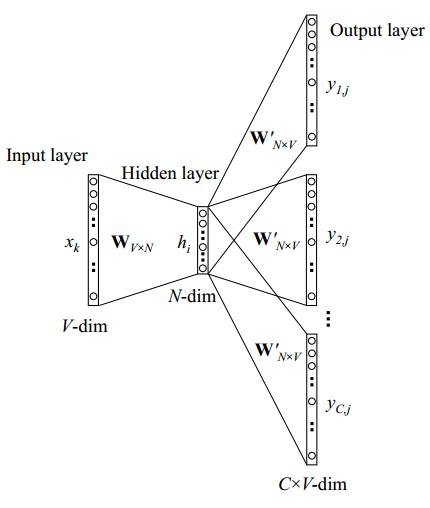
\includegraphics[width=70mm, height=70mm]{skipgram.jpg}
\caption{Skip Gram Model(Figure from Mikolov et al. (2013b)) \label{fig:skipgram}}
\end{figure}

%\subsection{tf-idf}
%Let $D=d_1, d_2, d_3....d_N$ be $N$ documents under study and $T=t_1, t_2, t_3,....t_M$ be the $M$ unique terms in these documents, then each document can be represented as a $M$-dimensional vector:\\
%$t_d=\{tf_1,tf_2,tf_3,...tf_M\}$\\
%$tf-idf$ weights discounts the frequency of terms based on their importance to a particular document in the entire document set collection under consideration. This is done as follows:
%\begin{center}
%$tfidf(d,t)=tf(d,t) \times \log(\frac{|D|}{df(t)})$ 
%\end{center}
%Here $df(t)$ is the number of documents in which term $t$ appears.

\subsection{Method}
The heart of the methodology lies in generating word vectors from the raw text. For this purpose we first trained skip-gram model on the Hindi dataset. As an output, we now have a $n$-dimensional vector representation for each word in the corpus. So given a sentence/document, we have averaged out the vectors to create a single vector for that particular sentence/document. This vector averaging is inspired by Mikolov et al. (2013b) and Levy et al. (2014) in which they have shown that many relational similarities can be recovered by means of vector arithmetic in the embedded space. This models the sentence/document in a high dimensional space.
%The preprocessing step was removal of few words based on their frequency in the corpus, both very high frequency and very low frequency words were pruned. This stop word pruning was not done in all experiments.\\
We also trained our model on the Hindi Wikipedia dump to create vector representations for words. The previous two vectors were concatenated to create another feature set for training purpose.

%\underline{\emph{Algorithm}}
%\begin{enumerate}
%\setlength{\itemsep}{0.5pt}
%\item Input a Hindi text corpus containing several sentences
%\item Train skip-gram model to obtain vector representation of words
%\item Average-out vectors for a given sentence/document
%\item Obtain tf-idf vector for each sentence/document in the corpus
%\item Concatenate vectors of step 3 and step 4 to obtain a feature set for a training instance
%\item Train linear SVM with $m$-fold cross validation to create a classifier
%\end{enumerate}

\section{Experiment Setup}
This section describes the corpus used in our experiment along with different experiment models and parameters. In all the experiments, we did 20-fold cross validation to calculate classification accuracy using linear SVM.
\subsection{Corpus}
We experimented on two Hindi review datasets. One is the Product Review dataset (LTG, IIIT Hyderabad) containing 350 Positive reviews and 350 Negative reviews. The other is a Movie Review dataset (CFILT, IIT Bombay) containing 127 Positive reviews and 125 Negative reviews. Similarly, for English, we trained on IMDB movie review dataset (Maas et al.(2013)) which consists of 25,000 positive and 25,000 negative reviews.\\
We also trained our skip-gram model on Hindi Wikipedia text dump (approx. 290MB) containing around 24M words with 724K words in the vocabulary. This provided us with good embeddings due to larger size and contents from almost all domains.

\subsection{Word Embeddings}
The quality of word vectors can be evaluated when they are compared with words which are closer to them semantically and syntactically. This can be accomplished by taking cosine similarity of each word with every other word in the vocabulary and outputting top few words which have greater cosine similarity. The other is to use tSNE~\cite{Maaten:08} which helps in visualizing high-dimensional data by giving each data point a location in a two or three-dimensional map. In our experiment, we took 5K words and plotted them with tSNE to highlight how these word vectors represent semantic and syntactic relations among words.

\begin{figure}[ht!]
\centering
\includegraphics[width=80mm]{tsne.pdf}
\caption{t-SNE visualization of Hindi Words in high dimensional space \label{fig:5K_hindi_zoom}}
\end{figure}

Figure \ref{fig:5K_hindi_zoom} gives a closer look into few clusters which depicts the relation between words in high dimensional space. Figure \ref{fig:5K_hindi_zoom1} shows that words such as {\dn mO\8{j}d} and {\dn uplND} are closer to each other but farther from words such as {\dn \31EwyAdA} and {\dn aEDk} which are closer to each other.

%\begin{figure*}[ht]
%\begin{minipage}[b]{0.31\linewidth}
%\centering
%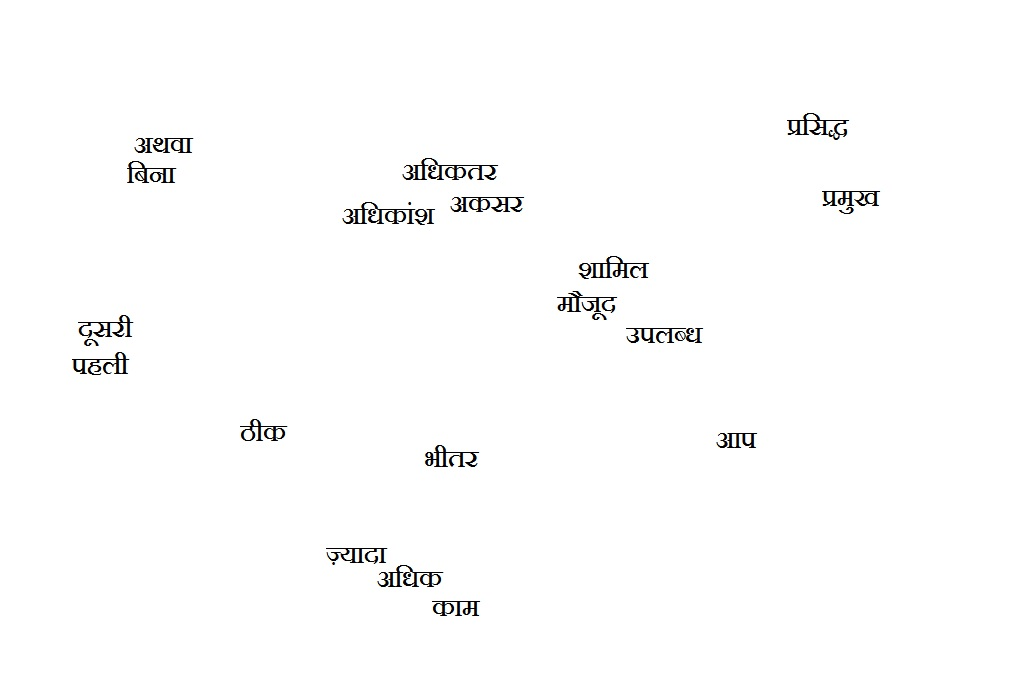
\includegraphics[width=\textwidth]{5K_hindi_zoom1.jpg}
%\caption{default}
%\label{fig:figure1}
%\end{minipage}
%\hspace{0.35cm}
%\begin{minipage}[b]{0.31\linewidth}
%\centering
%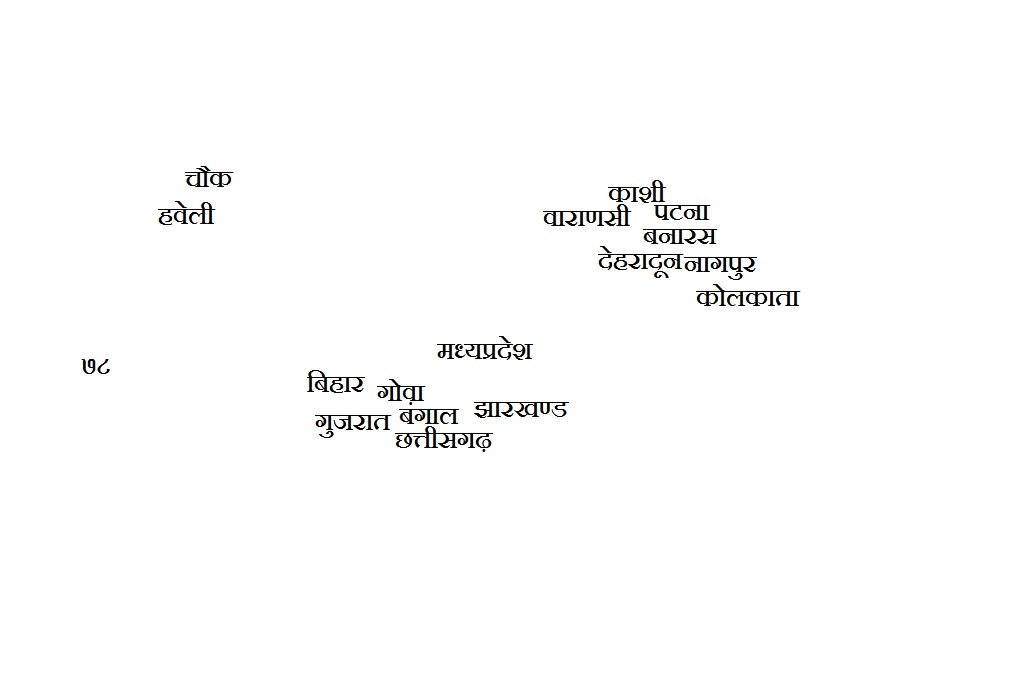
\includegraphics[width=\textwidth]{5K_hindi_zoom2.jpg}
%\caption{default}
%\label{fig:figure2}
%\end{minipage}
%\hspace{0.35cm}
%\begin{minipage}[b]{0.31\linewidth}
%\centering
%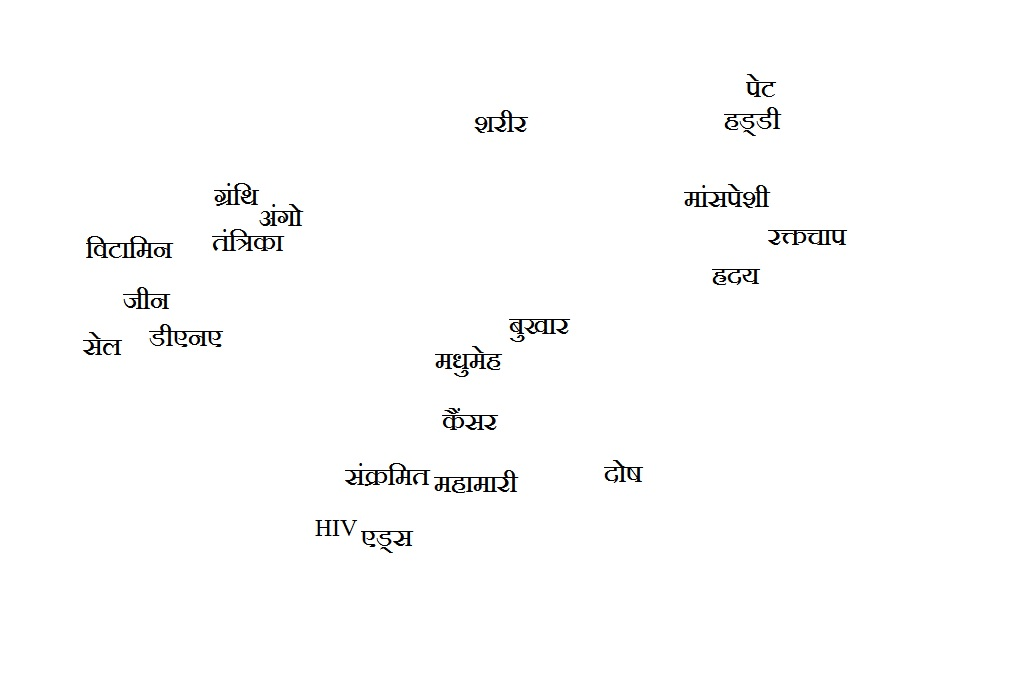
\includegraphics[width=\textwidth]{5K_hindi_zoom3.jpg}
%\caption{default}
%\label{fig:figure3}
%\end{minipage}
%\end{figure*}


\begin{figure}[ht!]
\centering
\subfigure[]{
            \label{fig:5K_hindi_zoom1}
            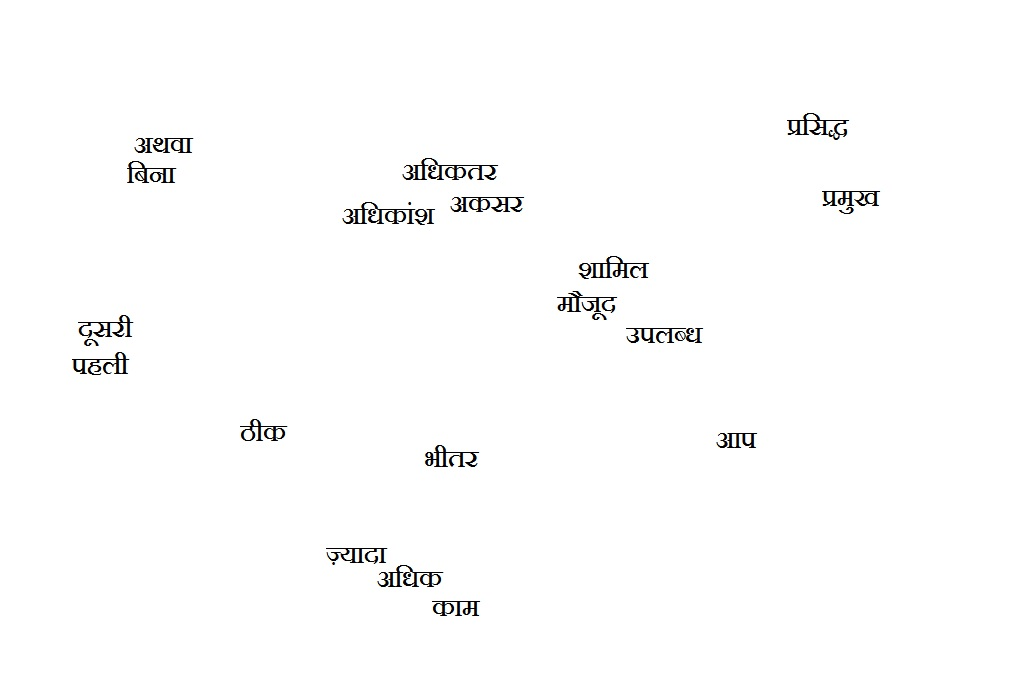
\includegraphics[width=0.4\textwidth]{5K_hindi_zoom1.jpg}
}
\subfigure[]{
            \label{fig:5K_hindi_zoom2}
            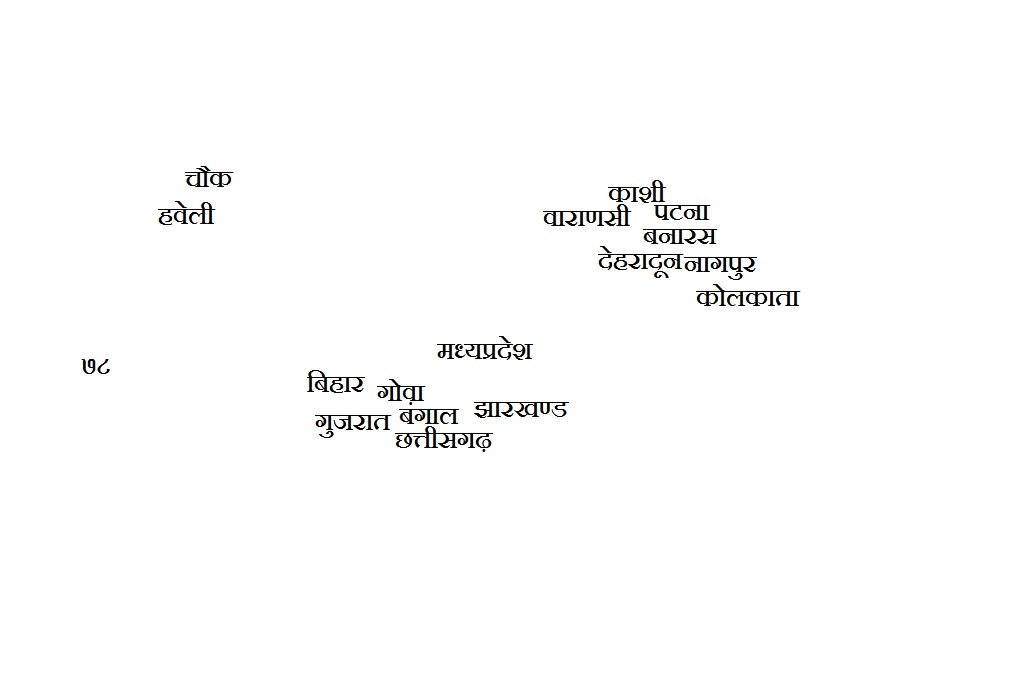
\includegraphics[width=0.4\textwidth]{5K_hindi_zoom2.jpg}
}
%\subfigure[]{
%            \label{fig:5K_hindi_zoom3}
%            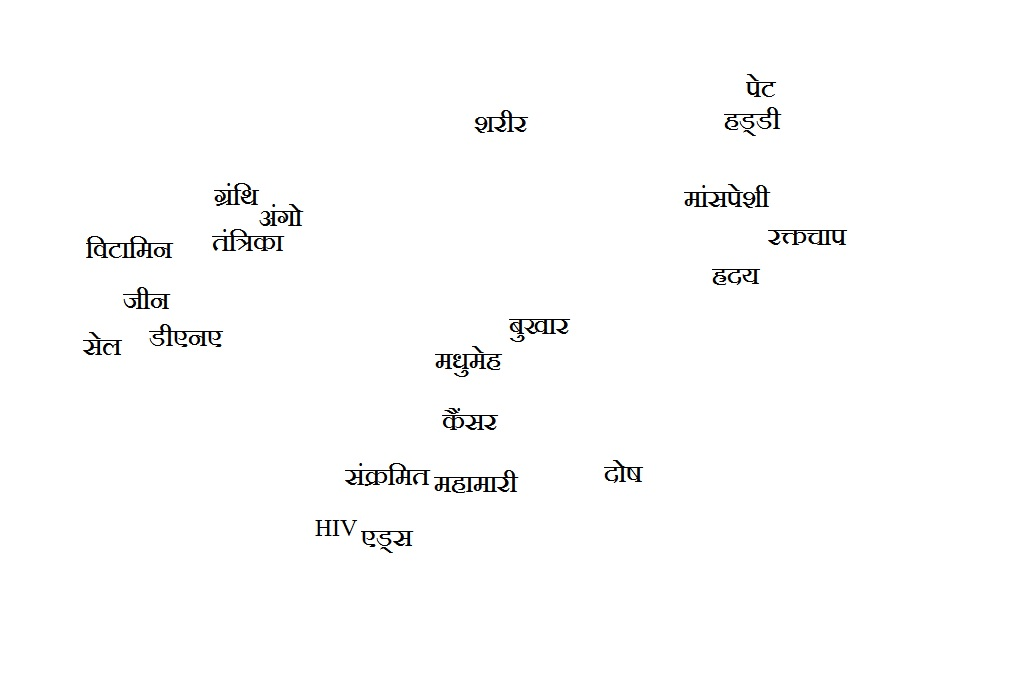
\includegraphics[width=0.4\textwidth]{5K_hindi_zoom3.jpg}
%}
\caption{A closer look at few clusters in the tSNE visualization\label{fig:5K_hindi_zoom}}
\end{figure}


\subsection{Skip-Gram and \emph{tf-idf} based Word Vectors}
In this experiment, we first generated 300-dimensional word vectors by training skip-gram model on both review corpus. The context size was taken as 5. We then averaged-out word vectors for each document to create document vectors. This now acts as a feature set for that particular document.
We also created \emph{tf-idf} vectors for each document. This can be seen as a vector representation of that particular document. We then concatenated these document vectors with document vectors obtained after averaging-out word vector of each document. In this case, the dimension of each word vector obtained from skip-gram training was 500.

%\subsection{Skip-Gram and \emph{tf-idf} based Word Vectors without stop-words}
%In this experiment, we filtered out stop-words on the basis of their frequency in the corpus. Words which had very high or very low frequency were pruned as they had negligible contribution to the %%sentiment polarity of a document. This is a noise-reduction step and gives better results.

\section{Results}

Table 1 is a summary of results which we and others have obtained on the IMDB dataset.
\begin {table}[H]
\small
\begin{tabular}{ | p{5.5cm} | l | }
\hline
\textbf{Features} & \textbf{Accuracy} \\ \hline
Maas et al.(2011) & 88.89\\ \hline
Paragraph Vector (Le and Mikolov(2014)) & 92.58\\ \hline
WordVector Averaging+Wiki (Our Method) & 87.56\\ \hline
\end{tabular}
\caption {IMDB Movie Review Dataset}
\end{table}

Table 2 represents the results which we have obtained on the Product Review Dataset and Movie Review Dataset using three different techniques for feature set construction. There has been a large improvement in accuracy when we include \emph{tf-idf} features along with word vectors. 
%We see that there is a slight improvement in accuracy on both datasets once we remove stop-words.
\begin {table}[H]
\small
\begin{tabular}{ | p{3cm} | l | l | }
\hline
\textbf{Features} & \textbf{Accuracy(1)} & \textbf{Accuracy(2)} \\ \hline
WordVector Averaging & 78.0 & 79.62\\ \hline
WordVector+tf-idf & 90.73 & 89.52\\ \hline
WordVector+tf-idf without stop words & \textbf{91.14} & \textbf{89.97}\\ \hline
\end{tabular}
\caption {Accuracy(1):Product Review Dataset and Accuracy(2): Movie Review Dataset}
\end{table}

Table 3 and 4 compares our best method(on Product and Movie Review Datasets respectively) with various other methods which have performed well using techniques such as \emph{tf-idf}, subjective lexicon, etc.

\begin {table}[H]
\small
\begin{tabular}{ | p{3cm} | p{2.2cm} | l | }
\hline
\textbf{Experiment} & \textbf{Features} & \textbf{Accuracy} \\ \hline
Word Vector with SVM (Our method) & tf-idf with word vector & \textbf{91.14}\\ \hline
Subjective Lexicon (Bakliwal et al.(2012)) & Simple Scoring & 79.03\\ \hline
Hindi-SWN Baseline (Arora et al.(2013)) & Adjective and Adverb presence & 69.30\\ \hline
\end{tabular}
\caption {Comparison of Approaches: Product Review Dataset}
\end{table}


\begin {table}[H]
\small
\begin{tabular}{ | p{3cm} | p{2.1cm} | p{1.3cm} | }
\hline
\textbf{Experiment} & \textbf{Features} & \textbf{Accuracy} \\ \hline
Word Vector with SVM (Our method) & tf-idf; word vector & \textbf{89.97}\\ \hline
In language using SVM (Joshi et al.(2010)) & tf-idf & 78.14\\ \hline
MT Based using SVM (Joshi et al.(2010)) & tf-idf & 65.96\\ \hline
Hindi-SWN Baseline (Arora et al.(2013)) & Adj. and Adv. presence & 68.40\\ \hline
\end{tabular}
\caption {Comparison of Approaches: Movie Review Dataset}
\end{table}

Table 5 shows the top few similar words for certain words from the corpus with cosine similarity as a distance metric. 
%The words which have higher cosine similarity tend to be semantically and syntactically related.
\begin {table}[H]
\small
\begin{tabular}{ | l | l | l | }
\hline
\textbf{{\dn aQCA}} & \textbf{{\dn{KrAb}}} & \textbf{{\dn ByAnk}} \\ \hline
{\dn b\7{h}t} & {\dn EnrAsAjnk} & {\dn By\306wkr}\\ \hline
{\dn \7{s}pr} & {\dn kM)or} & {\dn BFqZ}\\ \hline
{\dn k\?vl} & {\dn nA\7{)}k} & {\dn ByAvh}\\ \hline
{\dn itnA} & {\dn bdtr} & {\dn avsAd}\\ \hline
\end{tabular}
\caption {Sentiment Words and their Neighbors}
\end{table}


\section{Conclusion and Future Work}
Our word vector averaging method along with tf-idf outperforms all the existing methods. We also see that pruning stop words on the basis of frequency in the corpus also improves the accuracy slightly. The explanation for this improvement could be that words which have very high frequency tend to occur in most of the documents and they don't contribute to the sentiment. Words which have very low frequency can be considered as noise and can be safely pruned. For example, words such as {\dn EPSm} occur in 139/252 documents in Movie Review Dataset(55.16\%) and have no effect on sentiment information of a document. Similarly words such as {\dn Es\388wAT\0} occur in 2/252 documents in Movie Review Dataset(0.79\%). These words don't provide much information.\\
Our experiment results clearly indicate that proposed methods are helpful for much accurate sentiment classification. We expect that we can further improve our model by giving higher weights to adjectives and adverbs. Also, skip-gram model assumes that raw text for training is of large size. But in our case the training corpus was very small. So we can expect much better performance with our proposed approach if we have a much larger sentiment corpus.
%In future, one can come out with a weighted average heuristic to generate vectors for each document. 
We could provide a possible contribution in the construction of HSWN with the help of word vectors and their similarity. We could also incorporate word sense disambiguation and morphological variants for better accuracy while classification. The area of aspect-based sentiment analysis, also known as part-based sentiment analysis in Hindi is also unexplored which looks into several constituents of a document and classify their sentiment polarity individually.

\section*{Acknowledgements}
We thank LTG, IIIT Hyderabad and CFLT, IIT Bombay for providing us with the datasets. We also thank Computer Science and Engineering Department, IIT Kanpur for providing us with all the resources for the successful execution of this work.

% include your own bib file like this:
%\bibliographystyle{acl}
%\bibliography{acl2014}

\begin{thebibliography}{40}

%\bibitem[\protect\citename{Ahmad \bgroup et al.\egroup }2006]{Ahmad:06}
%Ahmad Khurshid, David Cheng, and Yousif Almas.
%\newblock 2006.
%\newblock Multi-lingual sentiment analysis of financial news streams.
%\newblock {\em In Proc. of the 1st Intl. Conf. on Grid in Finance}

\bibitem[\protect\citename{Joshi \bgroup et al.\egroup }2010]{Joshi:10}
Aditya Joshi, AR Balamurali, and Pushpak Bhattacharyya.
\newblock 2010.
\newblock A Fall-back Strategy for Sentiment Analysis in Hindi: a Case Study.
\newblock {\em International Conference on Natural language Processing (ICON)}

\bibitem[\protect\citename{Matilal }1990]{Matilal:90}
Bimal Krishna Matilal.
\newblock 1990.
\newblock The word and the world: India's contribution to the study of language.
\newblock {\em Oxford University Press, USA}

\bibitem[\protect\citename{Ohana \bgroup et al.\egroup }2009]{Ohana:09}
Bruno Ohana, and Brendan Tierney.
\newblock 2009.
\newblock Sentiment Classification of Reviews Using SentiWordNet.
\newblock {\em 9th. IT \& T Conference}

\bibitem[\protect\citename{Tang \bgroup et al.\egroup }2014]{Tang:14}
Duyu Tang, Furu Wei, Bing Qin, Ming Zhou, and Ting Liu.
\newblock 2014.
\newblock Building Large-Scale Twitter-Specific Sentiment Lexicon: A Representation Learning Approach.
\newblock {\em COLING},

\bibitem[\protect\citename{Huang \bgroup et al.\egroup }2012]{Huang:12}
Eric~H Huang, Richard Socher, Christopher~D Manning, and Andrew~Y Ng
\newblock 2012.
\newblock Improving Word Representations via Global Context and Multiple Word Prototypes.
\newblock {\em Annual Meeting of the Association for Computational Linguistics (ACL)},
   abs
   
\bibitem[\protect\citename{Mitchell \bgroup et al.\egroup }2008]{Mitchell:08}
Jeff Mitchell, and Mirella Lapata.
\newblock 2008.
\newblock Vector-based Models of Semantic Composition.
\newblock {\em JMLR},
   08/236.244
   
\bibitem[\protect\citename{Pennington \bgroup et al.\egroup }2014]{Pennington:14}
Jeffrey Pennington, Richard Socher, and Christopher~D. Manning.
\newblock 2014.
\newblock Glove: Global vectors for word representation.
\newblock {\em EMNLP},
   12/abs

\bibitem[\protect\citename{Turian \bgroup et al.\egroup }2010]{Turian:10}
Joseph Turian, Lev Ratinov, and Yoshua Bengio.
\newblock 2010.
\newblock Word representations: a simple and general method for semi-supervised learning.
\newblock {\em Proceedings of the 48th Annual Meeting of the Association for Computational Linguistics},
   12/384.394

\bibitem[\protect\citename{Maaten \bgroup et al.\egroup }2008]{Maaten:08}
L.J.P. van der Maaten, and G.E. Hinton.
\newblock 2008.
\newblock Visualizing High-Dimensional Data Using t-SNE.
\newblock {\em JMLR},
   08/2579.2605

\bibitem[\protect\citename{Mittal \bgroup et al.\egroup }2013]{Mittal:13}
Namita Mittal, Basant Agarwal, Garvit Chouhan, Nitin Bania, and Prateek Pareek.
\newblock 2013.
\newblock Sentiment Analysis of Hindi Reviews based on Negation and Discourse Relation.
\newblock {\em In the proceedings of 11th Workshop on Asian Language Resources, (in conjunction with IJCNLP -2013)},
   13/45.50
   
\bibitem[\protect\citename{Medagoda \bgroup et al.\egroup }2013]{Medagoda:13}
Nishantha Medagoda, Subana Shanmuganathan, and Jacqueline Whalley.
\newblock 2013.
\newblock A Comparative Analysis of Opinion Mining and Sentiment Classification in non-English Languages.
\newblock {\em International Conference on Advances in ICT for Emerging Regions (ICTer)},
   13/144.148

%\bibitem[\protect\citename{Chirawichitchai \bgroup et al.\egroup }2014]{Chirawichitchai:14}
%Nivet Chirawichitchai.
%\newblock 2014.
%\newblock Emotion Classification of Thai Text based Using Term weighting and Machine Learning Techniques.
%\newblock {\em 11th International Joint Conference on Computer Science and Software Engineering (JCSSE)}

\bibitem[\protect\citename{Levy \bgroup et al.\egroup }2014]{Levy:14}
Omer Levy, and Yoav Goldberg.
\newblock 2014.
\newblock Linguistic Regularities in Sparse and Explicit Word Representations.
\newblock {\em In Proceedings of the Eighteenth Conference on Computational Natural Language Learning},
   14/171.180

\bibitem[\protect\citename{Arora \bgroup et al.\egroup }2012]{Arora:12}
Piyush Arora, Akshat Bakliwal, and Vasudeva Varma.
\newblock 2012.
\newblock Hindi Subjective Lexicon Generation using WordNet Graph Traversal.
\newblock {\em International Journal of Computational Linguistics and Applications},
   3.1/25.39

\bibitem[\protect\citename{Collobert \bgroup et al.\egroup }2008]{Collobert:08}
Ronan Collobert, Jason Weston, Leon Bottou, Michael Karlen, Koray Kavukcuoglu, and Pavel Kuksa.
\newblock 2008.
\newblock Natural Language Processing (Almost) from Scratch.
\newblock {\em J. Mach. Learn. Res.},
   12/2493.2537

\bibitem[\protect\citename{Sharma \bgroup et al.\egroup }2014]{Sharma:14}
Richa Sharma, Shweta Nigam, and Rekha Jain.
\newblock 2014.
\newblock Opinion Mining In Hindi Language: A Survey.
\newblock {\em CoRR},
   abs/1404.4935
   
\bibitem[\protect\citename{Socher \bgroup et al.\egroup }2013]{Socher:13}
Richard Socher, Alex Perelygin, Jean~Y. Wu, Jason Chuang, Christopher~D. Manning, Andrew~Y. Ng, and Christopher Potts.
\newblock 2013.
\newblock Recursive deep models for semantic compositionality over a sentiment treebank.
\newblock {\em EMNLP},
  abs/1631.1642.
  
\bibitem[\protect\citename{Socher \bgroup et al.\egroup }2012]{Socher:12}
Richard Socher, Brody Huval, Christopher~D. Manning, and Andrew~Y. Ng.
\newblock 2012.
\newblock Semantic compositionality through recursive matrix-vector spaces.
\newblock {\em Proceedings of the 2012 Joint Conference on Empirical Methods in Natural Language Processing and Computational Natural Language Learning},
  abs/1201.1211.


\bibitem[\protect\citename{Johnson \bgroup et al.\egroup }2014]{Johnson:14}
Rie Johnson, and Tong Zhang.
\newblock 2014.
\newblock Effective Use of Word Order for Text Categorization with Convolutional Neural Networks.
\newblock {\em arXiv preprint},
  abs/1412.1058.

\bibitem[\protect\citename{Landauer \bgroup et al.\egroup }2003]{Landauer:03}
Thomas~K. Landauer, Darrell Laham, and Peter~W. Foltz.
\newblock 2003.
\newblock Automated scoring and annotation of essays with the Intelligent Essay Assessor.
\newblock {\em Automated essay scoring: A cross-disciplinary perspective},
  abs/87.112.

\bibitem[\protect\citename{Landauer \bgroup et al.\egroup }1997]{Landauer:97}
Thomas~K. Landauer, and Susan~T Dumais.
\newblock 1997.
\newblock A solution to Plato's problem: The latent semantic analysis theory of the acquisition, induction, and representation of knowledge.
\newblock {\em Psychological Review},
  104.2/211.240.

\bibitem[\protect\citename{Mikolov \bgroup et al.\egroup }2013]{Mikolov:13a}
Tomas Mikolov, Ilya Sutskever, Kai Chen, Gregory~S. Corrado, and Jeffrey Dean.
\newblock 2013.
\newblock Distributed Representations of Words and Phrases and their Compositionality.
\newblock {\em Advances in Neural Information Processing Systems},
  26/3111.3119.

\bibitem[\protect\citename{Mikolov \bgroup et al.\egroup }2013]{Mikolov:13b}
Tomas Mikolov, Kai Chen, Gregory~S. Corrado, and Jeffrey Dean.
\newblock 2013.
\newblock Efficient Estimation of Word Representations in Vector Space.
\newblock {\em CoRR},
  abs/1301.3781.

\bibitem[\protect\citename{Mikolov \bgroup et al.\egroup }2013]{Mikolov:13c}
Tomas Mikolov, Quoc~V. Le, and Ilya Sutskever.
\newblock 2013.
\newblock Exploiting similarities among languages for machine translation.
\newblock {\em arXiv preprint },
  abs/1309.4168.
   

\bibitem[\protect\citename{Zou \bgroup et al.\egroup }2013]{Zou:13}
Will~Y. Zou, Richard Socher Weston, Daniel Cer, and Christopher~D. Manning.
\newblock 2013.
\newblock Bilingual Word Embeddings for Phrase-Based Machine Translation.
\newblock {\em EMNLP},
   13/1393.1398
   
\end{thebibliography}

\end{document}
